\section{Design}\label{sec: Design}
In this section the design and decisions that where made to achieve the laboratory are discussed.

\subsection{Part I - RGB LED Driver}\label{subsec: Jupyter Notebook}
From project description, create the RGB LED color mixer using the ipywidgets integer or float slider. In theory, you should be able to create an infinite amount of colors with the combination of red, blue, and green LEDs. However,
with digital electronics, we are limited to the width of the driving data bus or processing system to create the colors. \\

• Create individual methods for enabling/disabling RED, GREEN and BLUE color of the RGB LED.\\

• PWM functionality for color mixing of the RGB LED.\\

• Create 3 color mixing sliders using ipywidgets. One slider per color (R-G-B).\\

• Create toggle buttons for all four of the green LEDs using ipywidgets.\\

• Create a way to set a flashing rate of the green LEDs using ipywidgets.\\

• Create a neat and organized GUI for all of the LED functionality. \\

First make a back up of all files that are to be modified. The files saved are \_\_init\_\_.py, base.py, and rgbled.py. This is done with connecting a network drive to the Python Productivity for ZYNQ (PYNQ) platform and copy the files over to an computer. The reason to do so is that the files can not be accessed over the web browser. Listening \ref{lst: p1_2} shows the changes made in the init file. This file imports the renamed class myrgbled by startup of the kernel. Listing \ref{lst: p1_3} shows how the base file is modified so that instead of the original rgbled driver the modified driver myrbgbled is used.

\begin{lstlisting}[style=PythonStyle, language=Python, caption={Python code changed on line 45 of file \_\_init\_\_.py.},label=lst: p1_2]
from .myrgbled import MYRGBLED
\end{lstlisting}

\begin{lstlisting}[style=PythonStyle, language=Python, caption={Python code changed on line 99 of file base.py.},label=lst: p1_3]
self.rgbleds = ([None] * 4) + [pynq.lib.MYRGBLED(i)
                                     for i in range(4, 6)]
\end{lstlisting}

To save the on the computer modified driver file back on to the PYNQ platform an trick is needed due to the restricted access rights of the /lib folder. Listing \ref{lst: p1_1} shows how the terminal command that is used to copy (cp) the file from folder /PYNQ to /PYNQ/lib because the file can be copyed into folder /PYNQ.

\begin{lstlisting}[language=bash, caption={Jupiter Notebook terminal, copy a file.},label=lst: p1_1]
root@pynq:/home/xilinx# cp /home/xilinx/pynq/myrgbled.py /home/xilinx/pynq/lib/myrgbled.py
\end{lstlisting}
%\begin{wrapfigure}{r}{0.7\textwidth}
\begin{figure}[H]
	\centering
	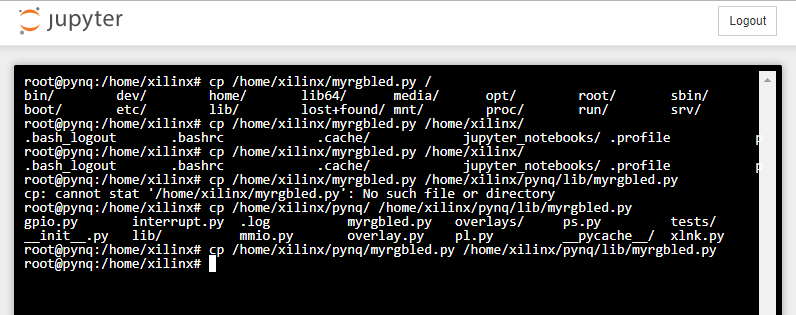
\includegraphics[width=\textwidth]{01_images/p1_terminal_cp}
	\caption{Jupiter Notebook terminal, copy a file.}
	\label{fig: part1_terminal}
\end{figure}
%\end{wrapfigure}

To the driver a method for pulse width modulation (PWM) is added, shown in Listing \ref{lst: p1_pwm_rgb}.
\begin{lstlisting}[language=python, caption={PWM for RGB LED.},label=lst: p1_pwm_rgb]

\end{lstlisting}

\subsection{Part II - LED Groove Bar}\label{subsec: Part II - LED Groove Bar}
The Groove LED Bar can be turned on in level increments from 0 to 10 where 0 is off and 10 all segments on. The brightness of the leds can be defined independently with an value from 0 to 3 where 0 is off, 1 is low, 2 is medium, and 3 is led brightness high. As graphical user interface (GUI) two integer slider are used SL1 and SL2 as shown in Figure \ref{fig: part2_output}. The source code is shown in Listing \ref{lst: Python Part 2} in Section \ref{subsec: Python code Listings Part II} of the appendix.

%\begin{wrapfigure}{r}{0.7\textwidth}
	\begin{figure}[H]
	\centering
	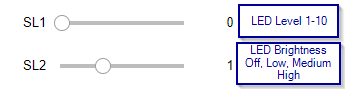
\includegraphics[width=0.6\textwidth]{01_images/p2_gui}
	\caption{Groove LED Bar program output.}
	\label{fig: part2_output}
	\end{figure}
%\end{wrapfigure}

\subsection{Part III - Music Synthesizer}\label{subsec: Part III - Music Synthesizer}
%In part two the Jupyter Notebook is used to program the game Let's Make a Deal. Is a game where a player can choose between four different doors. The computer decides behind which door win is placed.\\
%\\
%You can do the following to control the game:\\
%\\
%Button 0 pressed: \hfil       Door 1\\
%Button 1 pressed:   \hfil     Door 2\\
%Button 2 pressed: \hfil       Door 3\\
%Button 3 pressed: \hfil       Door 4\\
%\\
%Switch 0 on:   \hfil          Exit program\\
%Switch 1 on:    \hfil         Exit program\\
%\\
%Figure \ref{fig: part2_output} shows the console output shown in the web browser after executing the file with "Run All" and multiple rounds of choosing a door.
%%\begin{wrapfigure}{r}{0.7\textwidth}
%	\begin{figure}[H]
%	\centering
%	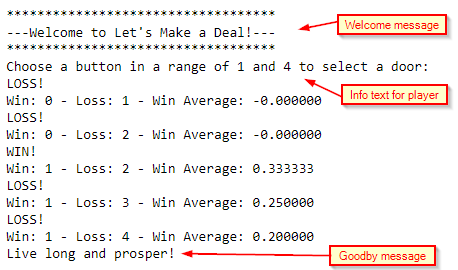
\includegraphics[width=0.8\textwidth]{01_images/part2_output.PNG}
%	\caption{Let's Make a Deal program output.}
%	\label{fig: part2_output}
%	\end{figure}
%%\end{wrapfigure}
%
%\subsection{Part III - Jupyter Notebook GUI using ipywidgets }
%The description of part three of the lab is as followed. 
%
%A Jupyter Notebook is not limited to just text output. By using the iPywidgets library, an interactive GUI can be
%created to interact with the I/O of the PYNQ board. For more information on ipywidgets, you can refer to the
%document “ipywidgets\_Userguide.pdf” available on the course website.
%
%Figure \ref{fig: part3_screen} shows the view programmed for part three which is used to control the LEDs. The first four buttons control LED zero to three and the status is shown with a label below the button. The two sliders control the RGB LEDs and can be used to change the color of each LED independently. Further more it shows how GUI elements are embedded in code and will appear after the cell where the display function is called. This gives the user an interesting interfacing option where he can adjust a code snipe and only execute the cell instead of the entire program.
%
%\begin{figure}[H]
%	\centering
%	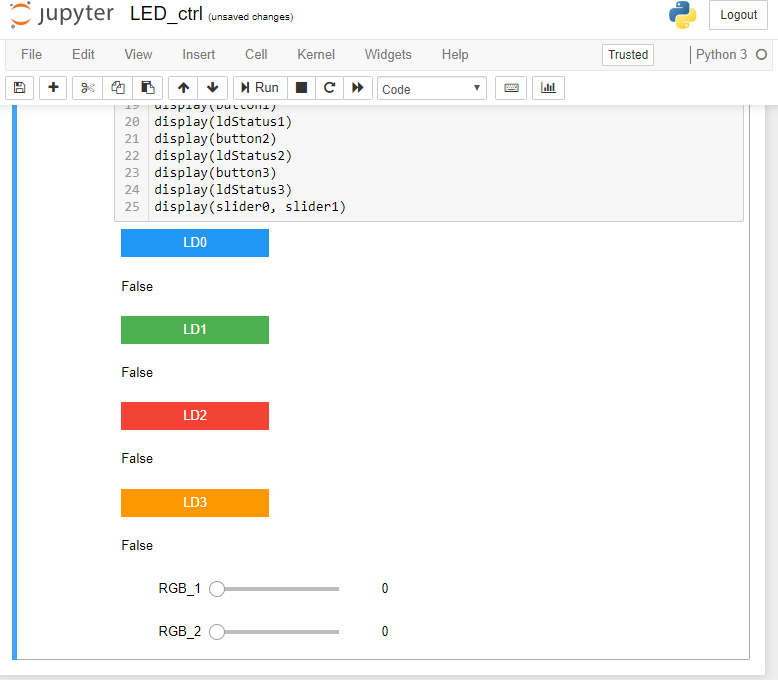
\includegraphics[width=0.9\textwidth]{01_images/part3_screen.PNG}
%	\caption{Buttons and slider for LED control.}
%	\label{fig: part3_screen}
%\end{figure}
%
%%\begin{lstlisting}[ caption={Error log saved as log\_error.txt file.},label=lst: Error log]
%%Thu Nov  1 01:32:15 2018 ATM program starts 
%%Thu Nov  1 01:32:33 2018 Error! Make sure you only use numbers from 0-9 in PIN
%%Thu Nov  1 01:32:35 2018 Error! Make sure you only use numbers from 0-9 in PIN
%%Thu Nov  1 01:32:38 2018 Error! Make sure you only use numbers from 0-9 in PIN
%%Thu Nov  1 01:32:47 2018 Program Closed
%%Thu Nov  1 01:33:15 2018 ATM program starts 
%%Thu Nov  1 01:33:34 2018 Program Closed
%%Thu Nov  1 01:33:37 2018 ATM program starts 
%%Thu Nov  1 01:33:54 2018 Invalid PIN!
%%Thu Nov  1 01:33:59 2018 Program Closed
%%Thu Nov  1 01:39:03 2018 ATM program starts 
%%Thu Nov  1 01:39:26 2018 Withdraw amount too big or not anouth balance
%%Thu Nov  1 01:39:31 2018 Withdraw amount too big or not anouth balance
%%Thu Nov  1 01:40:22 2018 Program Closed
%%Thu Nov  1 01:40:29 2018 ATM program starts 
%%Thu Nov  1 01:40:50 2018 Program Closed
%%Thu Nov  1 11:06:25 2018 ATM program starts 
%%Thu Nov  1 11:06:58 2018 Program Closed
%%Thu Nov  1 11:13:43 2018 ATM program starts 
%%Thu Nov  1 11:21:39 2018 Withdraw amount too big or not anouth balance
%%Thu Nov  1 11:21:44 2018 Program Closed
%%\end{lstlisting}
%
%%
%%An example code example for a empty tkinter window is shown in Listing \ref{lst: Python tkinter example code to create an empty window}.
%%\begin{lstlisting}[style=PythonStyle, language=Python, caption={Python tkinter example code to create an empty window.},label=lst: Python tkinter example code to create an empty window]
%%# import module
%%import tkinter as tk
%%
%%# define class with an empty main window
%%my_class(tk.Frame)
%%    def __init__(self, master=None):
%%		self.main_window = master
%%		self.main_window.title("ATM Bank Me")
%%
%%# instanciate class		
%%root = tk.Tk()
%%class_instance = my_class(root)
%%class_instance.main_window.mainloop()
%%
%%\end{lstlisting}
%%
%%An example code example for a canvas is shown in Listing \ref{lst: Python tkinter example code canvas}.
%%\begin{lstlisting}[style=PythonStyle, language=Python, caption={Python tkinter example code to create a canvas.},label=lst: Python tkinter example code canvas]
%%	#Make canvaas child of root
%%	canvas = tk.Canvas(master = main_window, width = 500, height = 300, bg = 'green')
%%	canvas.pack(side = 'top', fill = 'both', expand = 'yes')
%%\end{lstlisting}
%%An example code example for a frame is shown in Listing \ref{lst: Python tkinter example code for a frame}.
%%\begin{lstlisting}[style=PythonStyle, language=Python, caption={Python tkinter example code for a frame.},label=lst: Python tkinter example code for a frame ]
%%	# A frame is an invisible widget that holds other widgets. This frame goes 
%%	# on the right hand side of the window and holds the buttons and Entry widgets.
%%	self.frameControl = tk.Frame(master = main_window, width=500, height=100, background="green")
%%	self.frameControl.pack(side = tk.TOP,fill=tk.BOTH, ipady = 50)
%%\end{lstlisting}
%%
%%An example code example for a button and callback is shown in Listing \ref{lst: Python tkinter example code for a Button}. The call back opens a pop up message box with a title and a text message that can be used to inform a user about an event as example. Furthermore it contains code for an Entry and a Label widget.
%%\begin{lstlisting}[style=PythonStyle, language=Python, caption={Python tkinter example code for a Button with callabck that opens a message box.},label=lst: Python tkinter example code for a Button]
%%	# callback for button 
%%    def messagebox(self): 
%%		tk.messagebox.showinfo('Title','Text Message')
%%	# Button
%%	# With command = lambda: self.callback(arg1, arg2) a command with arguments is possible
%%	# without being executed at once on instantiation of the class.
%%    btTEST = tk.Button(master = self.frameControl, text = "Test", command = self.messagebox) 
%%    btTEST.pack(side = tk.LEFT, anchor='w', ipadx=20)   
%%    # Entry
%%    # with .bind('<return>', self.handler ) an callback can be restiered 
%%    # which would be executed on a return key press as further example
%%    enDeposit = tk.Entry(master = self.frameControl)
%%    enDeposit.pack(side = tk.TOP, anchor='w', ipadx=20, expand=True)
%%    enDeposit.insert(0, '$0') # set default value  
%%    # Label
%%    # A label can also be used a s placeholder to maintain order with using of .pack()
%%    lbBalanceAmount = tk.Label(master = self.frameControl, text='balance')
%%    lbBalanceAmount.pack(side = tk.TOP, anchor='w', ipadx=20, expand=True)
%%\end{lstlisting}
%%
%%
%%\subsection{Turtle}\label{subsec: Turtle}
%%According to \href{https://docs.python.org/3.3/library/turtle.html?highlight=turtle}{docs.python.org/3.3/library/turtle}, Turtle graphics is a popular way for introducing programming to kids. It was part of the original Logo programming language developed by Wally Feurzig and Seymour Papert in 1966.
%%Imagine a robotic turtle starting at (0, 0) in the x-y plane. After an import turtle, give it the command turtle.forward(15), and it moves (on-screen!) 15 pixels in the direction it is facing, drawing a line as it moves. Give it the command turtle.right(25), and it rotates in-place 25 degrees clockwise.
%%
%%The Bank Me Logo of the ATM is animated with turtle that allows a simple and fast way for a simple animation. Listening \ref{lst: Python turtle example code} shows an example code that uses turtle to draw the letter 'B'.
%%
%%\begin{lstlisting}[style=PythonStyle, language=Python, caption={Python turtle example code for a letter 'B'.},label=lst: Python turtle example code]
%%import turtle
%%
%%self.t = turtle.RawTurtle(canvas) # creatse a canvas to draw on
%%screen = self.t.getscreen() # returns the screen object 
%%# print(t.Screen().screensize()) 
%%
%%# This sets the lower left corner to 0,0 and the upper right corner to 600,600. 
%%screen.setworldcoordinates(0,0,250,200)
%%screen.bgcolor("green")
%%
%%# With the lines below, the "turtle" will look like a dollar sign 
%%# and can be placed wit t.stamp().
%%screen.register_shape("dollar_resize.gif")
%%self.t.shape("dollar_resize.gif")
%%
%%# Animation
%%t.pencolor("#FFFFFF") # WHITE
%%t.pensize(2)
%%
%%t.penup()   # Regarding one of the comments
%%t.forward(10)
%%t.left(90)
%%t.forward(10)
%%t.pendown() # Regarding one of the comments
%%# writes the letter 'B'
%%t.right(90)
%%t.circle(40, 180)
%%t.right(180)
%%t.circle(40, 180)
%%t.stamp()
%%\end{lstlisting}
%%
%%\subsection{ATM machine}\label{subsec: ATM machine }
%%\begin{wrapfigure}[21]{r}{0.48\textwidth}
%%	\centering
%%	\vspace{-1cm}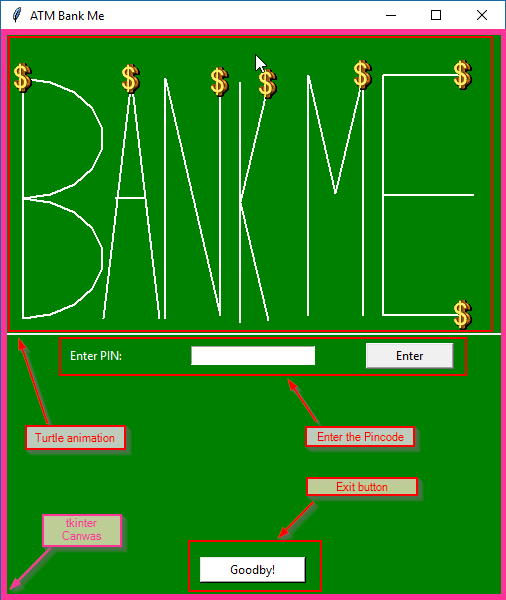
\includegraphics[width=0.48\textwidth]{01_images/gui_pin.PNG}
%%	\caption{GUI at start time after animation is done.}
%%	\label{fig: gui_pin}
%%\end{wrapfigure}
%%The ATM gui was build with tkinter and turtle. The error log and receipt print out is made with file I/O. The logic because it of simple logic flow could be drastically reduced compared to the previous lab. Therefore, no additional class was written. A complete code listening can be found in the appendix Section \ref{subsec: Python code Listings}. 
%%
%%Figure \ref{fig: gui_pin} shows the program after the animation is done and the user ask to enter the his personal identification number (PIN). After the pin has been entered in the Entry field the user can press the Enter button which will call the PIN verification method. Notice, that with the Goodbye button the program can be closed at any time. 
%%
%%As the user entered a valid PIN the pin entry objects are forgotten and destroyed because there is no need anymore for them. Instead the welcome message is shown and the objects to make a withdraw deposit and balance appear. By making an entry in one of the Entry fields for deposit or withdraw and pressing the button the user can either withdraw an amount of money from his account, not more then it contains or deposit amount of money.
%%
%%\begin{figure}[H]
%%	\centering
%%	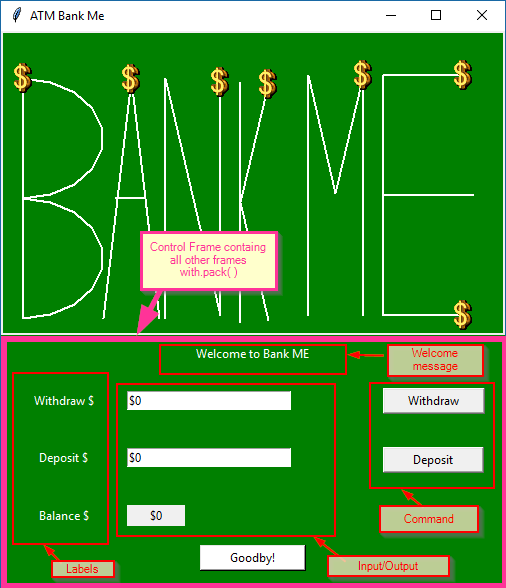
\includegraphics[width=0.5\textwidth]{01_images/gui.PNG}
%%	\caption{GUI after successful PIN entry.}
%%	\label{fig: gui}
%%\end{figure}
%%
%%
%%The following listening shows the error log output file content. This can be easily used to check which errors has been tested or for debugging. The error log is continuously appended into a text file and has to be managed manually. This could be automated with a script. 
%%\begin{lstlisting}[ caption={Error log saved as log\_error.txt file.},label=lst: Error log]
%%Thu Nov  1 01:32:15 2018 ATM program starts 
%%Thu Nov  1 01:32:33 2018 Error! Make sure you only use numbers from 0-9 in PIN
%%Thu Nov  1 01:32:35 2018 Error! Make sure you only use numbers from 0-9 in PIN
%%Thu Nov  1 01:32:38 2018 Error! Make sure you only use numbers from 0-9 in PIN
%%Thu Nov  1 01:32:47 2018 Program Closed
%%Thu Nov  1 01:33:15 2018 ATM program starts 
%%Thu Nov  1 01:33:34 2018 Program Closed
%%Thu Nov  1 01:33:37 2018 ATM program starts 
%%Thu Nov  1 01:33:54 2018 Invalid PIN!
%%Thu Nov  1 01:33:59 2018 Program Closed
%%Thu Nov  1 01:39:03 2018 ATM program starts 
%%Thu Nov  1 01:39:26 2018 Withdraw amount too big or not anouth balance
%%Thu Nov  1 01:39:31 2018 Withdraw amount too big or not anouth balance
%%Thu Nov  1 01:40:22 2018 Program Closed
%%Thu Nov  1 01:40:29 2018 ATM program starts 
%%Thu Nov  1 01:40:50 2018 Program Closed
%Thu Nov  1 11:06:25 2018 ATM program starts 
%Thu Nov  1 11:06:58 2018 Program Closed
%Thu Nov  1 11:13:43 2018 ATM program starts 
%Thu Nov  1 11:21:39 2018 Withdraw amount too big or not anouth balance
%Thu Nov  1 11:21:44 2018 Program Closed
%\end{lstlisting}
%\newpage
%Figure \ref{fig: printed_receipt} shows the receipt output generated by the program and opened in notepad by exiting the program by clicking the "Goodby!" button.
%\begin{figure}[H]
%	\centering
%	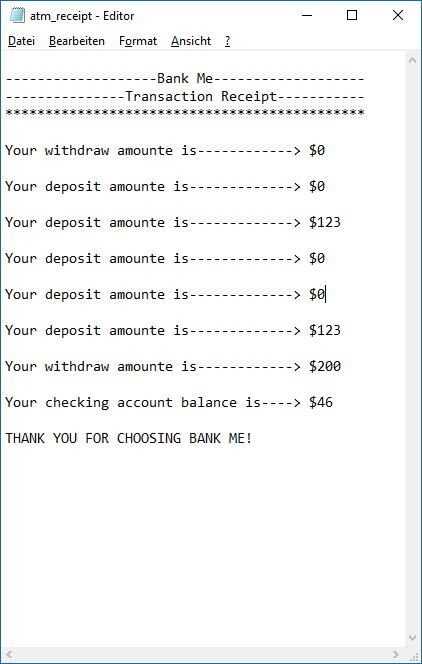
\includegraphics[width=0.5\textwidth]{01_images/printed_receipt.PNG}
%	\caption{Printed receipt.}
%	\label{fig: printed_receipt}
%\end{figure}
%
%Further work would be to write a better GUI class and separate logic and GUI a more distinguishably. 